\documentclass[10pt]{article}
\usepackage{CJKutf8}
\usepackage{hyperref}
\usepackage{graphicx}
\usepackage{textgreek}

% can create colorful boxes, for warning p.ex.
\usepackage[most]{tcolorbox}

% making the text of the report sans serif
\renewcommand{\familydefault}{\sfdefault}

% solve the issue when there is a dollar sign
% in a listing. Uses $\dollar$ instead
\newcommand{\dollar}{\mbox{\textdollar}}

\title{Setting up and using micro-ROS the Nucleo-144 \\[1ex] \large \begin{CJK}{UTF8}{min}南山大学\end{CJK}}
\date{}
\author{Vincent Conus}

\begin{document}
 
\maketitle

\begin{figure}[h]
  \centering
  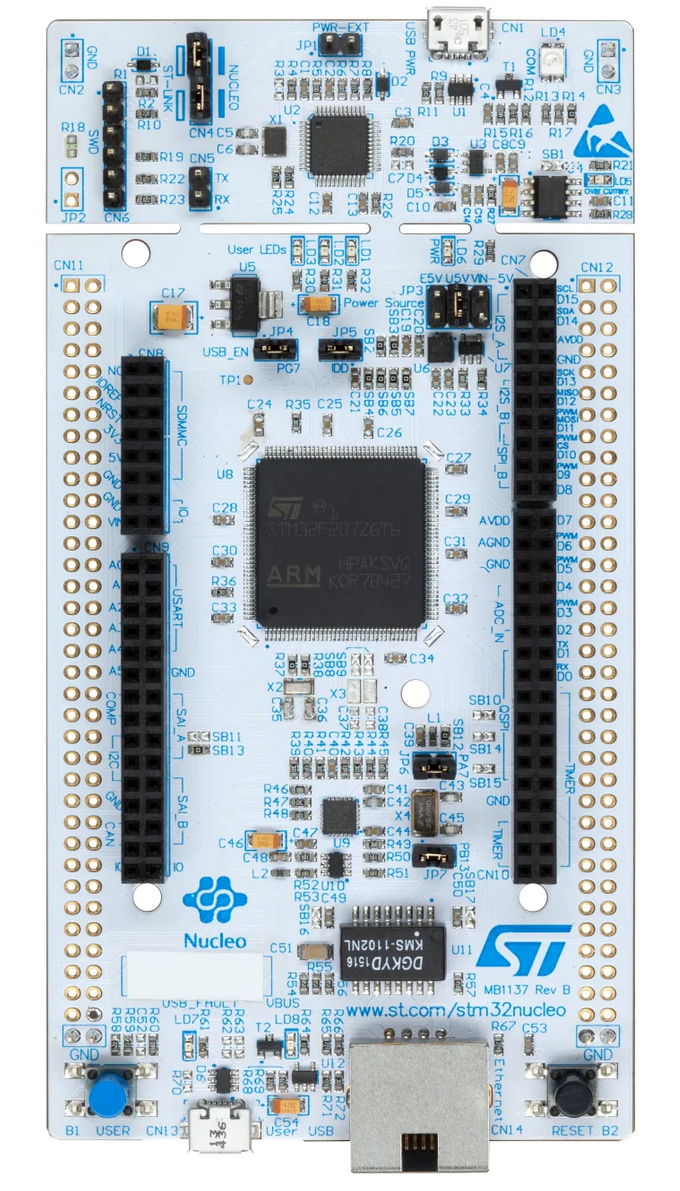
\includegraphics[width=0.5\textwidth]{./img/board.png}
\end{figure}

\pagebreak
%--------------------------------------------------------------------------------------
\section{Introduction and motivation}
Being a widely available board from ST and with an official support for micro-ROS, the Nucleo-144 is a great board as an intermediate step on the journey to have a ROS2 ecosystem running on a system like the \href{https://gitlab.com/nitrogen8m/documentation}{Nitrogen8M} with an heterogeneous cores setup.\\
Running a micro-ROS instance on this board is a useful goal in the overall project, as it will
allow me to test the ``standard'' use-case of that technology.\\
Later on, the goal will be to be able to run the DDS system over RPMsg.

%--------------------------------------------------------------------------------------
\section{Blinking a LED}
\label{sec:blinking-led}
When working with a microcontroller, this is always the first step to be taken
in order to know that the board is working and that our toolchain is properly
configured to upload a firmware to the board.

\subsection{STM32CubeIDE}
\label{sec:stm32cubeide}
Similarly to what presented in \href{https://gitlab.com/stm32mp157f-dk2/documentation}{my documentation for the STM32MP157F board}, the current Nucleo board projects can also be edited and loaded through serial connection from the \href{https://www.st.com/en/development-tools/stm32cubeide.html}{STM32 Cube IDE}. This tool has the advantage of being directly provided by ST and having a lot of available functionality for building and debugging project, however, such project are extremely inconvenient to move and are close to impossible to port.\\

Regardless, this is way we shall take for this guide, so as visible on the figure \ref{fig:ide} we are going to use the tool provided by ST to build and upload the firmware for our Nucleo board. The link in the previous paragraph explains how to install it.

\begin{figure}[h]
  \centering
  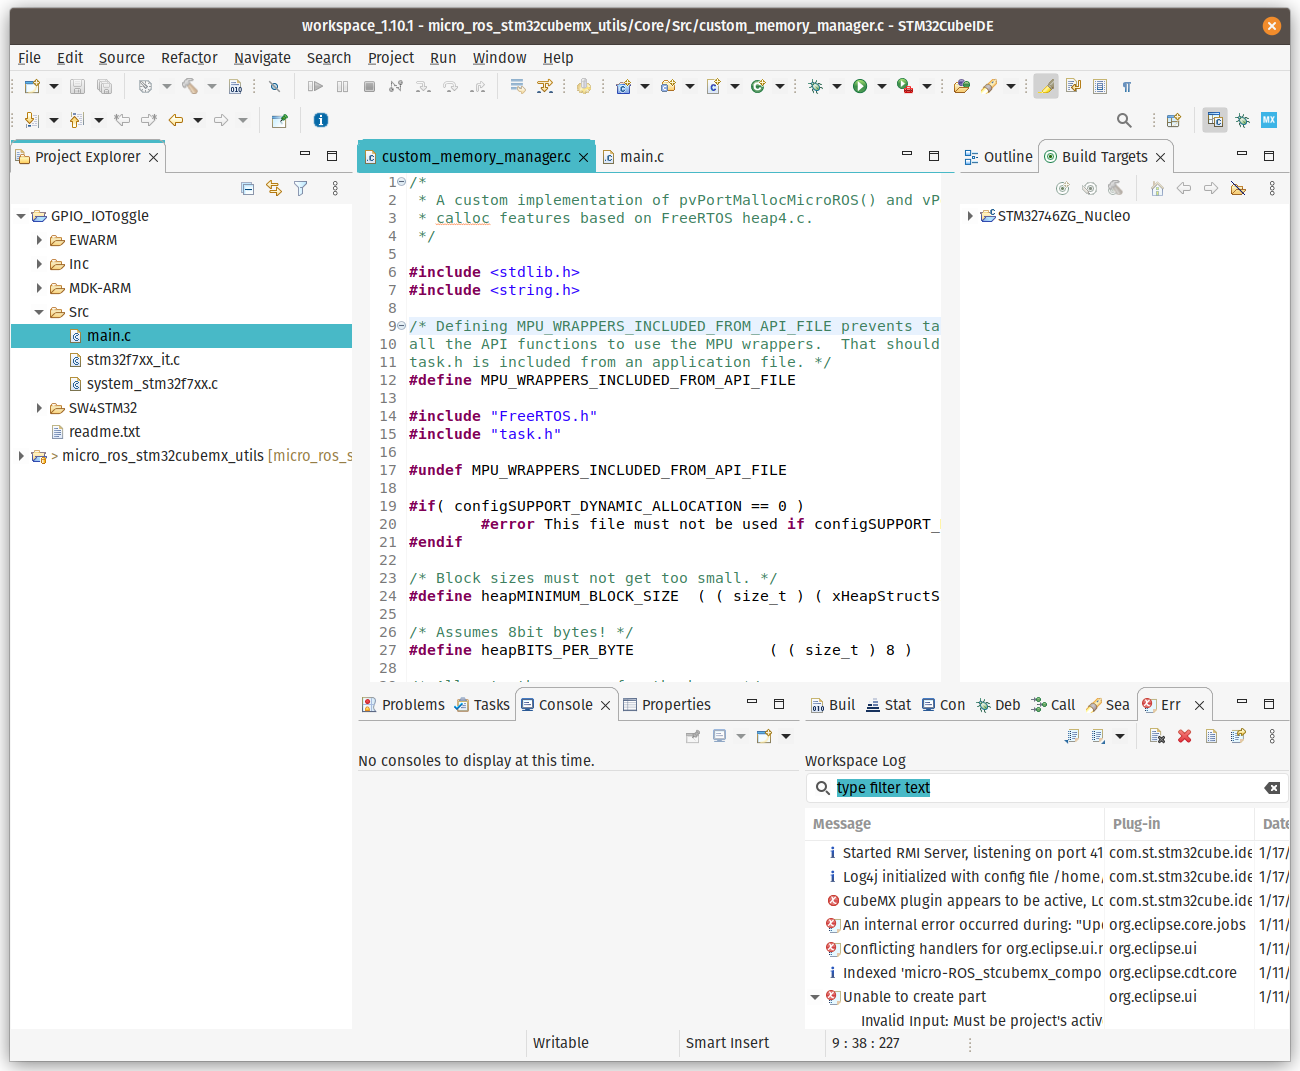
\includegraphics[width=0.8\textwidth]{./img/ide.png}
  \caption{The STM Cube IDE view, with a project opened}
  \label{fig:ide}
\end{figure}

\subsection{STM32F7 firmware package}
\label{sec:stm32f7-firmw-pack}
With the IDE ready to be used, we now have to get the firmware package for our board.
Since the Nucleo board we have is running a STM32F processor, we will need the similarly named pack.\\

The \href{https://www.st.com/content/st_com/en/products/embedded-software/mcu-mpu-embedded-software/stm32-embedded-software/stm32cube-mcu-mpu-packages/stm32cubef7.html}{STM32 cube F7 firmware package} is available at that link. Once the whole directory is download and decompressed, you can access all the template projects, navigating to the following directory (dependent on your actual version): \verb|./STM32Cube_FW_F7_vX.XX.X/Projects/STM32F746ZG-Nucleo/|. In particular, for our case as we want firstly to be able to blink an LED, we can navigate to further, into \verb|Examples/GPIO/GPIO_IOToggle|. This specific example is precisely what we want: a simple structure of a project that blinks the \verb|LED1| LED.

\subsection{Building and running the GPIO example}
\label{sec:build-runn-gpio}
The project downloaded as the F7 firmware, named \verb|GPIO_IOToggle| can be loaded into the IDE.
From the IDE interface, you can use \verb|File|, then \verb|Import...|, and then \verb|Existing Projects into Workspace|, as visible in the figure \ref{fig:import}. Then, as visible in the figure \ref{fig:project}, we can navigate to the \verb|GPIO_IOToggle| directory and open it as a project. You should have two nested project that can be imported here.

\begin{figure}[h]
  \centering
  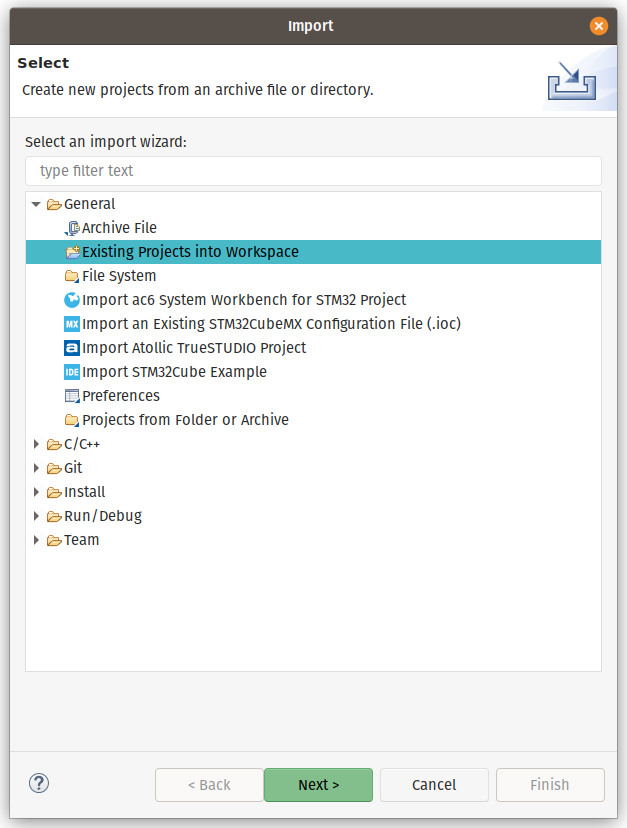
\includegraphics[width=.5\textwidth]{./img/import.png}
  \caption{Importing an existing project from the filesystem}
  \label{fig:import}
\end{figure}

\begin{figure}[!h]
  \centering
  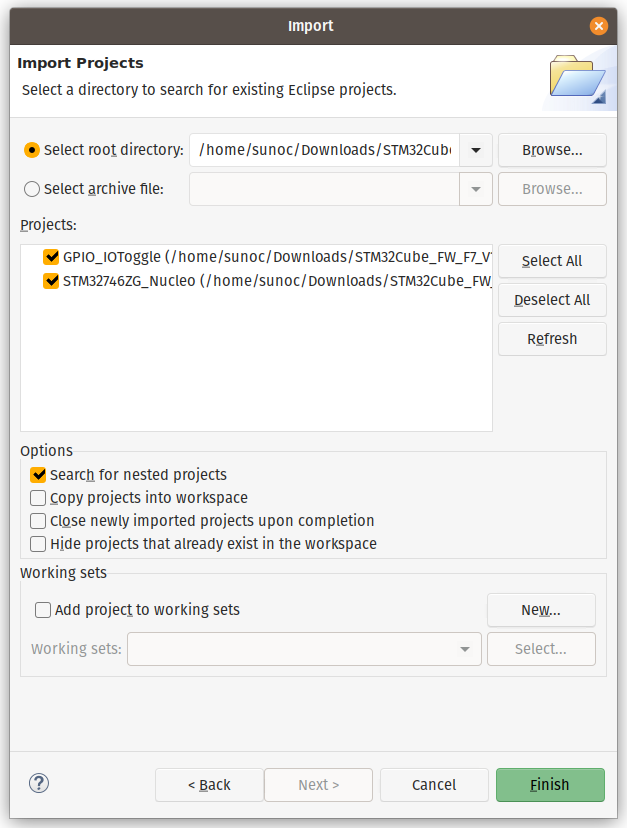
\includegraphics[width=.5\textwidth]{./img/project.png}
  \caption{Importing the nested GPIO projects}
  \label{fig:project}
\end{figure}

The project being imported, we can now see it's structure in the explorer of the IDE (figure \ref{fig:tree}). It also becomes clear here too why these STM Cube IDE are problematic to handle: even for such a simple task like the LED blink, a whole structure of inclusions and library that are elsewhere are needed.\\

However, with the Nucleo board plugged in the USB port of you computer, and by selecting the \verb|STM32746ZG| sub-project, you can build the example (hammer icon), and then run it (white arrow on a green dot icon).\\
As visible in the figure \ref{fig:toggle_led}, if you navigate around the line 90 of the \verb|main.c| file, you will find a delay function that takes some milliseconds in entry parameter. By changing that value, you are able to check if the code you are building is indeed being uploaded to the board.\\

With this setup, you should be able to build the example and having the LD1 LED on the top of your Nucleo board to blink.

\begin{figure}[h]
  \centering
  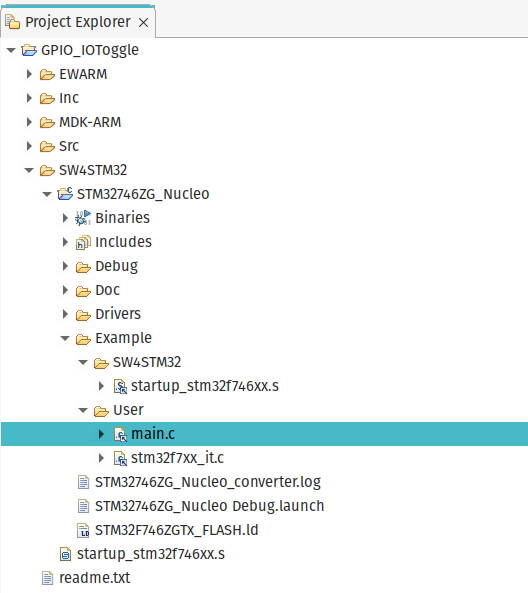
\includegraphics[width=.9\textwidth]{./img/tree.png}
  \caption{GPIO project structure}
  \label{fig:tree}
\end{figure}

\begin{figure}[!h]
  \centering
  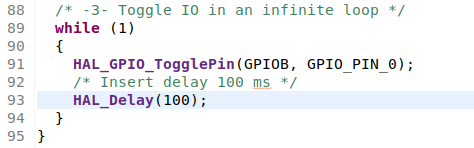
\includegraphics[width=.9\textwidth]{./img/toggle_led.png}
  \caption{``while'' loop with the toggling timing for the LD1 LED}
  \label{fig:toggle_led}
\end{figure}

\pagebreak
% --------------------------------------------------------------------------------------
\section{micro-ROS}
\label{sec:micro-ros}
Now we have a minimal project running on our Nucleo board, it's time to try, deploy and run a micro-ROS instance.
Deploying micro-ROS on a microcontroller is not a trivial task, as the firmware that is meant to be compiled and sent over must contain at least:
\begin{itemize}
\item The specific drivers for the board
\item A real-time operating system, most likely FreeRTOS
\item The micro-ROS layer itself
\item The program that will use this micro-ROS environment
\end{itemize}

Furthermore, it is every more hard to debug such deployment, since a micro-ROS is only visible as it communicates with a full-on ROS2 system.

\subsection{Local Linux micro-ROS running a ping-pong test app}
\label{sec:local-linux-micro}
The first step in the path of running micro-ROS, we should try to run a ping-pong application on my Linux machine.
Some instructions for this particular task are given on \href{https://micro.ros.org/docs/tutorials/core/first_application_linux/}{micro-ROS website}.
Alternatively, there is a \href{}{micro-ROS report prepared by Prof. Honda}, available on this very repository.\\

In this section of the report about the Nucleo board, I will present a tested, combined step-by-step guide on how to accomplish this task.\\

Docker is used in both guides to have a controlled environment to build and run these test tools.
It is then important to install it on your system (or even remotely). \href{https://docs.docker.com/engine/install/}{The official Docker documentation} is the way to go, and it depends on your operating system. Even on your desktop, the version you'd want is the ``server'' version, as it is more widely available and more lightweight. From here I will assume that you have a docker install handy.\\


The following commands will pull a ROS container, version \verb|foxy|, and name it \verb|ros_build|.
Then, we can execute \verb|bash|, as a way to open a terminal to the ``inside'' of the container.
\begin{tcolorbox}
\begin{verbatim}
sudo docker run -d --name ros_build -it --net=host -v \
     /dev:/dev --privileged ros:foxy
sudo docker exec -it ros_build bash
\end{verbatim}
\end{tcolorbox}


From inside the container, we can follow the micro-ROS wiki guide, as to have two micro-ROS nodes that can run a default ``ping-pong'' application, as a proof that the system works and that the instances are able to communicated with each other.\\
The following command list will pull the required firmware, build it, then build, setup and run the agents inside you Docker container:
\begin{tcolorbox}
\begin{verbatim}
. /opt/ros/$ROS_DISTRO/setup.\verb|bash|

mkdir microros_ws
cd microros_ws
git clone -b $ROS_DISTRO \
    https://github.com/micro-ROS/micro_ros_setup.git \
    src/micro_ros_setup

sudo apt update && rosdep update
rosdep install --from-paths src --ignore-src -y
sudo apt-get -y install python3-pip wget nano

colcon build
. ./install/local_setup.bash

ros2 run micro_ros_setup create_firmware_ws.sh host

ros2 run micro_ros_setup build_firmware.sh
. ./install/local_setup.bash

ros2 run micro_ros_setup create_agent_ws.sh
ros2 run micro_ros_setup build_agent.sh
. ./install/local_setup.bash

ros2 run micro_ros_agent micro_ros_agent udp4 --port 8888
\end{verbatim}
\end{tcolorbox}

Once your agent is running, you can open another terminal in your Docker (similarly to what was presented above: \verb|sudo docker exec -it ros_build bash|), and run the following commands to start the micro-ROS pingpong app:
\begin{tcolorbox}
\begin{verbatim}
. /opt/ros/$ROS_DISTRO/setup.bash
. ./install/local_setup.bash

export RMW_IMPLEMENTATION=rmw_microxrcedds

ros2 run micro_ros_demos_rclc ping_pong
\end{verbatim}
\end{tcolorbox}

Then in yet another terminal, you can \verb|bash| into your container and run the following commands to actually test the running pingpong application:
\begin{tcolorbox}
\begin{verbatim}
. /opt/ros/$ROS_DISTRO/setup.bash

ros2 topic echo /microROS/ping
\end{verbatim}
\end{tcolorbox}

If you see some nanosec timestamp with a \verb|frame_id| value, you are doing it right !

\subsection{micro-ROS on a microcontroller}
\label{sec:micro-ros-micr}
Now we know that we can build micro-ROS agents, the goal is to build a firmware for our Nucleo board that can talk to our PC via serial.
This should be possible following the \href{https://micro.ros.org/docs/tutorials/core/first_application_rtos/freertos/}{official guide} since the board is \href{https://micro.ros.org/docs/overview/hardware/}{officially supported}.\\


Similarly to the previous section, we will \verb|bash| into our ROS2 Docker. From here, we can  pull the firmware for the STM32 boards and run the setup scrips:
\begin{tcolorbox}
\begin{verbatim}
git clone -b galactic \
https://github.com/micro-ROS/micro_ros_stm32cubemx_utils.git \
/project

ros2 run micro_ros_setup create_firmware_ws.sh \
freertos nucleo_f746zg

ros2 run micro_ros_setup configure_firmware.sh \
ping_pong --transport serial

ros2 run micro_ros_setup build_firmware.sh

cp firmware/freertos_apps/microros_nucleo_f746zg_extensions/\
build/micro-ROS.bin /tmp/nucleo/
\end{verbatim}
\end{tcolorbox}

Now to have the local agent connecting to the topic, you can run the following command, and then plug-out and plug-in the usb cable:
\begin{tcolorbox}
\begin{verbatim}
ros2 run micro_ros_agent micro_ros_agent serial \
--dev /dev/ttyACM0
\end{verbatim}
\end{tcolorbox}

It is possible to view the Nucleo board as a mountable volume by plugging in the \verb|USB PWR| port to your machine. The \verb|/dev/sdX| will be mounted as something similar to \verb|/media/user/NODE_F746ZG|.\\
It is also an option to mount this device from inside a Docker, for example with the following:
\begin{tcolorbox}
\begin{verbatim}
mkdir /tmp/nucleo
mount /dev/sda /tmp/nucleo
\end{verbatim}
\end{tcolorbox}

We can then upload the firmware to the board by moving the \verb|.bin| to the mounted volume:
\begin{tcolorbox}
\begin{verbatim}
cp firmware/freertos_apps/\
microros_nucleo_f746zg_extensions/build/micro-ROS.bin \
/tmp/nucleo/
\end{verbatim}
\end{tcolorbox}

Now the firmware is flashed, we can create, build, setup the agent, run the app (remotely, through the \verb|/dev/ttyACME0|):
\begin{tcolorbox}
\begin{verbatim}
ros2 run micro_ros_setup create_agent_ws.sh

ros2 run micro_ros_setup build_agent.sh
. ./install/local_setup.bash

ros2 run micro_ros_agent micro_ros_agent serial \
--dev /dev/ttyACM0
\end{verbatim}
\end{tcolorbox}

Finally, for testing this application, you can bash into the Docker from another term and run these:
\begin{tcolorbox}
\begin{verbatim}
. /opt/ros/$ROS_DISTRO/setup.bash

ros2 topic echo /microROS/ping
\end{verbatim}
\end{tcolorbox}

\subsection{=TODO= Usage with N8M}
\label{sec:usage-with-n8m}
As the micro-ROS deployed system appear to work properly,it will become interesting
to make the board able to ``talk'' with my other Nitrogen8M ROS2 deployment.\\

This is a good exercise to see if everything works as expected, especially at
the DDS level.


\end{document}